\section{Лекція 6: Цикли}
 
 \subsection{Що таке цикл?} 
\begin{frame}
% \frametitle{Логічні висновки}
Цикли — оператори, які дозволяють повторювати код певну кількість разів.

\huge{цикл (умова):

~~~~операції
}

\normalsize Позначення:

\large{заголовок циклу:

~~~~тіло циклу
}


\end{frame}

\begin{frame}
\frametitle{Цикл while}
Визначимо суму чисел від 1 до N.

s = 0

i = 1 

N = 1000

while i <= N:

~~~~s += i

~~~~i += 1

Одноразове виконання тіла цикла називається ітерацією цикла.

\end{frame}

 \subsection{Оператори break та continue} 
\begin{frame}
% \frametitle{Цикл while}
\begin{itemize}
  \item break - дострокове завершення циклу.
  \item continue - пропуск однієї ітерації циклу.
  \item В блоці else йдуть команди, що виконуються після штатного завершення циклу.
\end{itemize}
\end{frame}

 \subsection{Цикл for} 
\begin{frame}
% \frametitle{Логічні висновки}
\huge{for змінна in ітератор:

~~~~операції
}

\vspace{1cm}
\normalsize 
У циклі for вказується змінна і низка значень, на які буде послатися змінна в різних ітераціях. Значення можуть бути задані списком, кортежем, рядком тощо. Значення, на які посилається змінна в циклі \underline{не змінюються} (для такої зміни слід звертатися до елементів за індексом).

\end{frame}

 \subsection{Функція range} 
\begin{frame}
% \frametitle{Логічні висновки}
Функція \texttt{range()} генерує ряд чисел у межах заданого діапазону. Можна визначити початок та кінець цього ряду, а також якою буде різниця між двома числами.

\begin{itemize}
  \item \texttt{range(stop)}
  \item \texttt{range(start, stop)}
  \item \texttt{range(start, stop, step)}
\end{itemize}
\end{frame}

\subsection{Приклади застосування циклу for} 
\begin{frame}
% \frametitle{Логічні висновки}
\begin{enumerate}
  \item 
  Розрахунок факторіалу натурального числа n:

\begin{center}
n! = 1*2*3*...*(n-1)*n
\end{center}
\item 
Відобразити ялинку:

*

**

***

****

*****

\item 
Задано список із цілих чисел. Треба замінити кожне двозначне число на нуль.
\end{enumerate}
\end{frame}

\subsection{Функція enumerate}
\begin{frame}
% \frametitle{Логічні висновки}
Іноді, при переборі об'єктів у циклі for, потрібно як отримати сам об'єкт, а й його порядковий номер. Це можна зробити за допомогою ітератора enumerate:

\huge{for i, el in enumerate(lst):

~~~~операції}
\end{frame}

\subsection{Ітератори} 
\begin{frame}
% \frametitle{Логічні висновки}
Об'єкт, що ітерується (iterable) - це об'єкт, який здатний повертати елементи по одному. Крім того, це об'єкт, з якого можна одержати ітератор.

Приклади об'єктів, що ітеруються:

\begin{itemize}
  \item всі послідовності: список, рядок, кортеж
  \item словники
  \item файли 
\end{itemize}
    
Ітератор використовується для одноразового перебору елементів об'єкту.
\end{frame}

\begin{frame}
% \frametitle{Логічні висновки}
Функція \texttt{iter()} повертає ітератор і створює об'єкт, який може перебиратися по одному елементу за раз.

Щоб отримати наступне значення з ітератора, використовується функцію \texttt{next()}. Не можна використовувати \texttt{next()} зі списком чи кортежем, але можна зробити список, кортеж або рядок ітератором (функцією \texttt{iter()}), а потім використати \texttt{next()}.

Якщо ітерований об'єкт пройдено до кінця, то застосування до нього функції \texttt{next()} призводе до помилки StopIteration.
\end{frame}

\subsection{Вкладені цикли} 
\begin{frame}
% \frametitle{Логічні висновки}
Вкладені цикли використовуються для роботи із вкладеними списками або із списками ітерованих об'єктів.

\huge{
for i in iterator\_1:

~~~~for j in iterator\_2:

~~~~~~~~operations
}
\end{frame}

\begin{frame}
% \frametitle{Логічні висновки}
Для транспонування вкладеного списку A  використовується програма:

% \texttt{
for i in range(N):

~~~~for j in range(i+1, N):

~~~~~~~~A[i][j], A[j][i] = A[j][i], A[i][j]
% }
\end{frame}

\begin{frame}
% \frametitle{Логічні висновки}
\begin{figure}
\begin{center}
 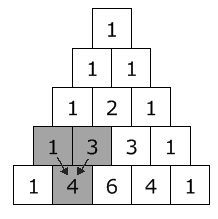
\includegraphics[width=0.4\textwidth]{pictures/pascal.png}
\caption{Трикутник Паскаля}
\label{pascal} 
\end{center}
\end{figure}
\end{frame}
